
% \pdfminorversion=4


\documentclass[conference]{journal}

\usepackage[normalem]{ulem}
\usepackage{amsmath}
% \usepackage[pdftex]{graphicx}
\usepackage{cite}
\usepackage{xspace}
\usepackage{tikz}
\usepackage{pgfplots}
\usepackage[per-mode=symbol]{siunitx}
\usepackage{booktabs}
\usepackage{tikzscale}
\usepackage{array}
\usepackage{amsmath,amsfonts,amssymb}
\usepackage{xcolor}

\usepackage{algorithm}
\usepackage[noend]{algpseudocode}

\newcommand*\circled[1]{\tikz[baseline=(char.base)]{
   \node[shape=circle,draw,inner sep=1pt] (char) {#1};}}

\newcommand{\bb}[1]{\mathbb{#1}}
\newcommand{\B}[1]{\mathbf{#1}}
\newcommand{\Bx}{\B{x}}
\newcommand{\Bv}{\B{v}}
\newcommand{\Bq}{\B{q}}
\newcommand{\BV}{\B{V}}
\newcommand{\Beta}{\boldsymbol{\eta}}
\newcommand{\Brho}{\boldsymbol{\rho}}

\newcommand{\xt}{{}^{t}\Bx}
\newcommand{\vt}{{}^{t}\dot{\Bx}}
\newcommand{\at}{{}^{t}\ddot{\Bx}}

\newcommand{\xtt}{{}^{t+\Delta t}\Bx}
\newcommand{\vtt}{{}^{t+\Delta t}\dot{\Bx}}
\newcommand{\att}{{}^{t+\Delta t}\ddot{\Bx}}

\newcommand{\M}{\bb{M}}
\newcommand{\C}{\bb{C}}
\newcommand{\K}{\bb{K}}


% correct bad hyphenation here
%\hyphenation{op-tical net-works semi-conduc-tor}
\begin{document}
	
	% paper title
	% Titles are generally capitalized except for words such as a, an, and, as,
	% at, but, by, for, in, nor, of, on, or, the, to and up, which are usually
	% not capitalized unless they are the first or last word of the title.
	% Linebreaks \\ can be used within to get better formatting as desired.
	% Do not put math or special symbols in the title.
	\title{Various Concepts of Modal Analysis and Model Reduction Methods}
	
	% author names and affiliations
	% use a multiple column layout for up to three different
	% affiliations
	\author{\IEEEauthorblockN{Alexandra Leukauf, Sebastian Thormann, Jan Valasek,  and Michael Zauner \textcolor{red}{email missing}
	 }
	\IEEEauthorblockA{Institute of Mechanics and Mechatronics\\Technical University of Vienna, Austria\\
	}}
	
	% make the title area
	\maketitle
	
	% As a general rule, do not put math, special symbols or citations
	% in the abstract
	\begin{abstract}
		With modal analysis it is possible to predict the dynamic behavior of a system, which is  important for the system's technical design. Another aspect is to minimize the computational effort of mathematical models in numeric simulations. By a reduction of the model's degrees of freedom an approximation to the original model can be computed. The goal of this paper is to provide an overview of common methods for modal analysis, including the free oscillation eigenvalue problem in time/frequency domain and model order reduction methods. With those the reduced model needs significantly less computation time and still shows accurate results.
	\end{abstract}
	
	% no keywords
	
	
	
	
	% For peer review papers, you can put extra information on the cover
	% page as needed:
	% \ifCLASSOPTIONpeerreview
	% \begin{center} \bfseries EDICS Category: 3-BBND \end{center}
	% \fi
	%
	% For peerreview papers, this IEEEtran command inserts a page break and
	% creates the second title. It will be ignored for other modes.
	\IEEEpeerreviewmaketitle
	
	\section{Introduction}
	Analyzing a system in terms of its eigenvalues and eigenvectors simplifies system analysis, and gives insight into dynamic system behavior.
	This modal analysis is used for e.g. the design of bridges and machine foundations, together with many other technical or mathematical applications. 
	
	The crash of the Tacoma-Narrows bridge is a great example to underline the importance of modal analysis. Due to high wind conditions, which excited the bridge close to its natural frequency, the bridge collapsed only four months after opening. 

	The natural frequencies of a system are the frequencies at which the system naturally tends to oscillate under disturbance. This  eigenfrequency depends primarily on structural properties like the mass and stiffness, but also on the boundary conditions. In case of a damped system the damping has also an influence on the characteristic frequencies. Each eigenfrequency has a corresponding mode shape (eigenvector), which can be seen as the deformed shape of the system at this specific frequency. 
	
	In this paper, the eigenfrequencies and eigenvectors of a mechanical multi-degree-of-freedom system are derived by solving the eigenvalue problem. The results are an indication on how the system will respond to dynamic excitations.
	
	In the first section the free-oscillation eigenvalue problem is derived and the most common numeric eigenvalue solvers are presented. The main topic of the second section is the solution of the equation of motion, which is investigated in time and frequency domain. Additionally Rayleigh and modal damping are considered. Finally in section three the transformation to modal coordinates is explained, as well as how to use and choose a modal subspace.
	
	\section{Free oscillation Eigenvalue problem}
	A mechanical system with $n$ degrees of freedom can be described by 
	\begin{equation}\label{motion eq}
	\textbf{M\"x}+\textbf{D\.{x}}+\textbf{Kx}=\textbf{f},
	\end{equation}
	where $\mathrm{\textbf{M}}$ is the mass matrix, $\mathrm{\textbf{D}}$ is the damping matrix and $\mathrm{\textbf{K}}$ is the stiffness matrix. All matrices are of the same dimension $n \times n$, whereas the forcing vector $\textbf{f}$ and the displacement vector $\textbf{x}$ have the size $n \times 1$. When considering the system's undamped free oscillation, damping and external forcing must be set zero, which leads to
	\begin{equation}
	\textbf{M\"x}+\textbf{Kx}=\textbf{0}.
	\end{equation}
	In order to solve this system of second order linear differential equations, a general solution of the form
	\begin{equation}
	\textbf{x}(t)=\Re\{\textbf{\^x}e^{\lambda t}\}
	\end{equation}
	is inserted into (\ref{motion eq}). Where $\lambda$ is the root of the characteristic equation, which is explained later. As a consequence, one obtains the free oscillation eigenvalue problem
	\begin{equation}
	[\textbf{K}+\lambda^2 \textbf{M}]\textbf{\^x}=0.
	\end{equation}
	Besides this quadratic eigenvalue problem, the general eigenvalue problem of the form
	\begin{equation}
	\textbf{A\^x}=\lambda\textbf{B\^x}
	\end{equation}
	and, of course, the standard eigenvalue problem
	\begin{equation}\label{standard}
	\textbf{A\^x}=\lambda\textbf{\^x}
	\end{equation}
	should also be mentioned. Sometimes it might be useful to convert the different types of eigenvalue problems to the standard form (\ref{standard}). One possibility to transform the quadratic eigenvalue problem to a generalized one is to introduce a new solution vector $\textbf{\^y}=\lambda\textbf{\^x}$, which leads to
	\begin{equation}
	\begin{bmatrix}
	\textbf{K} & \textbf{0} \\
	\textbf{0} & \textbf{I}
	\end{bmatrix}
	\begin{bmatrix}
	\textbf{\^x} \\
	\textbf{\^y}
	\end{bmatrix}
	=\lambda
	\begin{bmatrix}
	\textbf{-D} & \textbf{-M} \\
	\textbf{I} & \textbf{0}
	\end{bmatrix}
	\begin{bmatrix}
	\textbf{\^x} \\
	\textbf{\^y}
	\end{bmatrix}.
	\end{equation}
	This generalised problem again can be transformed further to the standard problem by left-multiplying with $\textbf{B}^{-1}$
	\begin{equation}
	\textbf{B}^{-1}\textbf{A\^x}=\lambda\textbf{\^x}.
	\end{equation}
	
	
	\section{Eigenvalue solvers}
	The goal of eigenvalue solvers is to find the eigenvalues $\lambda_i$ and their corresponding non-trivial eigenvectors $\textbf{\^x}_i$ of (\ref{standard}). An eigenvalue problem with $n$ degrees of freedom has $n$ non-trivial solutions if the characteristic equation
	\begin{equation}
	\det (\textbf{A}-\lambda\textbf{I})=0,
	\end{equation}
	is fulfilled. In order to get unique eigenvectors, $(\textbf{A}-\lambda\textbf{I})$ must not be singular, which can be achieved by setting constraints. 
	
	\subsection*{Vector Iteration}
	This algorithm is an appropriate solver for sparse matrices and only produces the biggest eigenvalue by its magnitude.  
	\begin{equation}
	\textbf{\^x}_\mathrm{k+1}=\frac{\textbf{A\^x}_\mathrm{k}}{\lVert \textbf{A\^x}_\mathrm{k} \rVert}
	\end{equation}
	Here, $\lVert \textbf{A\^x}_\mathrm{k} \rVert$ converges towards the largest eigenvalue, whereas $\textbf{\^x}_\mathrm{k+1}$ provides the corresponding eigenvector.
	
	\subsection*{Inverse Vector Iteration}
	The inverse vector iteration uses the same principle as vector iteration. However, considering the fact that $\lambda$ is an eigenvalue of $\textbf{A}$, then $\lambda-\sigma$ is an eigenvalue of $\textbf{A}-\sigma\textbf{I}$. Moreover, $\mu=\frac{1}{\lambda - \sigma} $ is an eigenvalue of the inverse $ (\textbf{A}-\sigma \textbf{I})^{-1}= \textbf{B}$. 
	Applying the vector iteration for $\textbf{B}$ 
	\begin{equation}
	\textbf{\^x}_\mathrm{k+1}=\frac{\textbf{B\^x}_\mathrm{k}}{\lVert \textbf{B\^x}_\mathrm{k} \rVert},
	\end{equation}
	one obtains the highest eigenvalue $\mu$ of $\textbf{B}$. Which corresponds to the eigenvalue of $\textbf{A}$ after the back-transformation
	\begin{equation}
	\lambda=\sigma+\frac{1}{\mu}.
	\end{equation}
	Setting the shift point $\sigma=0$, the solver computes the largest eigenvalue $\mu$ of $\textbf{B}$, which leads to the smallest eigenvalue $\lambda_1$. If the shift point $\sigma$ is chosen close enough to a desired $\lambda_i$, the solver delivers good results.
	
	\subsection*{Rayleigh Quotient Iteration}
	The Rayleigh quotient iteration is an inverse vector iteration with a prescribed shift point of
	\begin{equation}
	\sigma_{\mathrm{k}}=\frac{\textbf{\^x}_{\mathrm{k}}^\intercal\textbf{A\^x}_{\mathrm{k}}}{\textbf{\^x}_{\mathrm{k}}^\intercal\textbf{\^x}_{\mathrm{k}}},
	\end{equation}
	Setting the shift point $\sigma=0$, the solver computes the largest eigenvalue $\mu$ of $\textbf{B}$, which leads to the smallest eigenvalue $\lambda_1$. If the shift point $\sigma$ is chosen close enough to a desired $\lambda_i$, the solver delivers good results.
	
	\subsection*{Rayleigh Quotient Iteration}
	The Rayleigh quotient iteration is an inverse vector iteration with a prescribed shift point of
	\begin{equation}
	\sigma_{\mathrm{k}}=\frac{\textbf{\^x}_{\mathrm{k}}^\intercal\textbf{A\^x}_{\mathrm{k}}}{\textbf{\^x}_{\mathrm{k}}^\intercal\textbf{\^x}_{\mathrm{k}}},
	\end{equation}
	called Rayleigh quotient. This very efficient eigenvalue algorithm has high a rate of convergence.
	
	\subsection*{Gram-Schmid Process}
	With the Gram-Schmid process one can compute any higher eigenvectors $\textbf{\^x}_k,...,\textbf{\^x}_n$ of 
	$\textbf{A}$, if the lower eigenvectors $\textbf{\^x}_1$ to $\textbf{\^x}_{k-1}$ are known. Given an arbitrary linear independent basis $\textbf{v} _1, \textbf{v}_2, ..., \textbf{v}_n$, the Gram-Schmid algorithm constructs an orthogonal basis $\{\textbf{u}_1, \textbf{u}_2,..., \textbf{u}_n\}$ by computing 
	\begin{equation}
	\textbf{u}_{\mathrm{k}} = \textbf{v}_{\mathrm{k}} -\sum_{\mathrm{j=1}}^{\mathrm{k-1}}\mathrm{p}(\textbf{v}_{\mathrm{j}},\textbf{u}_{\mathrm{k}})
	\end{equation}
	with the projection of $v$ onto $u$
	\begin{equation}
	p(\textbf{v},\textbf{u})=\frac{\textbf{v}\textbf{u}}{\textbf{u}\textbf{u}}\textbf{u}.
	\end{equation}
	Now, $\textbf{u}_k$ can be used for the inverse vector iteration to calculate
	$\textbf{u}_\mathrm{k+1}=\frac{\textbf{Bu}_\mathrm{k}}{\lVert \textbf{Bu}_\mathrm{k} \rVert}$.
	
	\subsection*{QR-Algorithm}
	This algorithm uses the QR-decomposition
	\begin{equation}
	\textbf{A}_\mathrm{k}={\textbf{Q}_\mathrm{k}}{\textbf{R}_\mathrm{k}},
	\end{equation}
	where $\textbf{Q}_\mathrm{k}$ is a unitary matrix and $\textbf{R}_\mathrm{k}$ is an upper triangular matrix.
	This decomposition can be easily computed by any mathematical program like matlab, as well as by, for instance, the Gram-Schmid process. After iterating
	\begin{equation}
	\textbf{A}_\mathrm{k+1}={\textbf{R}_\mathrm{k}}{\textbf{Q}_\mathrm{k}},
	\end{equation}
	the matrix $\textbf{A}$ usually has an upper triangular form and its eigenvalues are located at the diagonal. This algorithm produces all the eigenvalues at once.
	 
	\subsection*{Subspace Iteration}
	The subspace iteration delivers only a subset $p<n$ of eigenvalues of $\textbf{A}$. Starting with an initial vector $\textbf{X}_k$, one computes
	\begin{equation}
	\textbf{Z}_{k+1}=\textbf{AX}_k
	\end{equation}
	and calculates the QR-decomposition of $\textbf{Z}_k$ by
	\begin{equation}
	\textbf{Z}_k=\textbf{X}_k\textbf{R}_k.
	\end{equation}
	The largest $p$ eigenvalues are located at the diagonal of $\textbf{R}_k$.
	
	
	
	\section{Time and frequency domain}
	We consider a linear time invariant system of ordinary differential equations (ODE) of the second order
	\begin{equation} \label{eq:2system}
	\M \ddot{\Bx} + \C \dot{\Bx} + \K \Bx = \B{f},
	\end{equation}
	where the initial conditions $\dot{\Bx}(t_0)=\B{v}_0$, $\Bx(t_0)=\Bx_0$ and the source term $\B{f}=\B{f}(t)$ are known. We focus on a structural dynamics problem where $\Bx=\Bx(t)$ denotes a generalized coordinates field which is deformed over time by a load $\B{f}$ and by the initial conditions. The parameters of this system are constant matrices which are well-known as mass $\M$, damping $\C$ and stiffness matrix $\K$.

	The beam in figure \ref{fig:beam} should serve as an example problem for the system described above. Its surface on the left is clamped and one corner on the right is loaded by a vertical force $\B{P}$. Assuming a small deflection compared to the size of the beam the \textit{Euler-Bernoulli Theory} can be applied and we can derive a system as stated in (\ref{eq:2system}). The parameter matrices can be found by using the finite element, the finite differences method or other methods to discretize homogeneous materials.

	\begin{figure}[h]
	\centering
	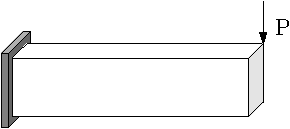
\includegraphics{./figures/beam.pdf}
	\caption{Clamped beam loaded by $\B{P}$}
	\label{fig:beam}
	\end{figure}

	We are interested in numerical methods which can be used to explain the dynamical phenomena of the deformations. There are direct and indirect time integration methods for calculating the dynamic behavior of a system.

	% The transient behavior can be analyzed by time integration which is expensive in computational resources. Since we consider a linear autonomous term of the differential equation system it depends on the source term, if we can use modal analysis directly to efficiently get answers on the frequency domain. Both methods will be explained and illustrated with the example at hand. In the next section an additional method combining both will be shown to achieve superior efficiency. 

	\subsection{Direct Time Integration}
	A time integration scheme is called direct when the equations are not transformed prior to the numerical integration. The basic idea is to satisfy (\ref{eq:2system}) only at discrete time intervals $\Delta t$. Explicit methods, such as Forward/Backward Euler or Runge-Kutta evaluate the system equations at the current time step to calculate the solution of $\Bx$ at the next time step. These are not necessarily stable for a given time discretization.

	Implicit methods, such as Newmark or Wilson-$\theta$, are stable and specialized for second order ODEs. These calculate the solution for the same time step as they evaluate the system equations. We focus on the Newmark method which makes the following assumptions
	% 
	\begin{equation} \label{eq:2newmark-asump}
	\begin{aligned}
	\vtt &= \vt 
	+ \Delta t \left((1-\delta)\; \at + \delta\;\att \right)\,,
	\\[.5em]
	\xtt &= \xt + \vt\;\Delta t
	+ \Delta t^2\;\left((0.5-\alpha) \; \at + \alpha\;\att \right)\,
	\end{aligned}
	\end{equation}
	% 
	or rewritten as
	% 
	\begin{equation} \label{eq:2newmark-asump-re}
	\begin{aligned}
	\att &= \frac{\xtt - \xt}{\alpha \Delta t^2} - \frac{\vt}{\alpha \Delta t} - \frac{2 \alpha \at}{1 - 2\alpha}\,,
	\\[.5em]
	\vtt &= \vt + \Delta t (1-\delta) \at + \delta \Delta t \att\,.
	\end{aligned}
	\end{equation}
	%
	The parameters $\alpha$ and $\delta$ determine how the acceleration is interpolated within one time step. Using $\delta=0.5$ and $\alpha=0.25$ corresponds to the approximation of a constant average acceleration.
	

	Plugging (\ref{eq:2newmark-asump}) in (\ref{eq:2system}) with the stated Newmark parameters we get
	% 
	\begin{equation} \label{eq:2newmark-solve}
	\widetilde{\K}\;\xtt = {}^{t+\Delta t}\widetilde{\B{f}}
	\end{equation}
	% 
	with the effective stiffness matrix
	% 
	\begin{equation} \label{eq:2newmark-K}
	\widetilde{\K} = \frac{4}{\Delta t^2} \M + \frac{2}{\Delta t} \C + \K
	\end{equation}
	% 
	and the effective load vector
	% 
	\begin{equation} \label{eq:2newmark-f}
	\begin{aligned}
	\widetilde{\B{f}} = {}^{t+\Delta t}{\B{f}}
	&+ \M \left( \frac{4}{\Delta t^2} \xt + \frac{4}{\Delta t} \vt + \at \right)
	\\
	&+ \C \left( \frac{2}{\Delta t} \xt + \vt \right)\,.
	\end{aligned}
	\end{equation}

	By applying the Newmark method to the dynamical problem from (\ref{eq:2system}) we arrived at (\ref{eq:2newmark-solve}) which has the same form as a static problem. Since (\ref{eq:2system}) can be interpreted as
	% 
	\begin{equation} \label{eq:2system-forces}
	\B{f}_\mathrm{M} + \B{f}_\mathrm{C} + \B{f}_\mathrm{K} = \B{f}\,,
	\end{equation}
	% 
	where $\B{f}_\mathrm{M}$ denotes the pseudo inertia, $\B{f}_\mathrm{C}$ the damping and $\B{f}_\mathrm{K}$ the stiffness force, the actual dynamic problem can be reformulated as a series of static problems in each time step. The basic steps are shown in algorithm \ref{newmark}.

	\begin{algorithm}
	\caption{Newmark time integration}\label{newmark}
	\begin{algorithmic}[1]
	\Procedure{Newmark}{$\M,\, \C,\, \K,\, \B{f}(t),\, \Delta t,\, t_\mathrm{end},\, {}^{0}\Bx,\, {}^{0}\dot{\Bx}$}
	\State ${}^{0}\ddot{\Bx} \gets 0$
	\State $\widetilde{\K} \gets \mathrm{evaluate} \; \circled{\ref{eq:2newmark-K}}$
	\ForAll{$t \in \{0,\,\Delta t,\,2\Delta t,\,\mathellipsis,\,t_\mathrm{end}\}$}
		\State ${}^{t+\Delta t}\widetilde{\B{f}} \gets \mathrm{evaluate} \; \circled{\ref{eq:2newmark-f}}$
		\State $\xtt \gets \mathrm{solve} \; \circled{\ref{eq:2newmark-solve}}$
		\State $\left(\att,\vtt\right) \gets \mathrm{evaluate} \; \circled{\ref{eq:2newmark-asump-re}}$
	\EndFor
	\EndProcedure
	\end{algorithmic}
	\end{algorithm}

	
	
	\section{Model order reduction}
	The goal of this section is to present methods on how to effectively reduce degrees of freedom of given systems. This leads then to a decrease of computational cost and time.
	
	\subsection{Modal basis}
	We consider again the system of differential equations of second order, which describes the motion of an elastic body
	\begin{equation} \label{eq:3system}
	\M \ddot{\Bx} + \C \dot{\Bx} + \K \Bx = \B{f}.
	\end{equation}
	Here we denoted mass, damping and stiffness matrix as $\M, \C, \K$, vector $\B{f}$ represents acting forces and the influence of Neumann boundary conditions and finally in the vector $\Bx$ are stored the unknown displacements of this system with $N$ degrees of freedom. The solution of associated quadratic eigenvalue problem reads
	\begin{equation} \label{eq:3eigs}
	(\K + \lambda \C + \lambda^2 \M) \Bv = \B{0},
	\end{equation}
	where $\lambda$ is a eigenvalue and $\B{v}$ is eigenvector corresponding to the eigenvalue $\lambda$. This problem has normally $n$ eigenvalues and eigenvectors. 
	
	The first key idea in this section is to change the coordinate system from a physical to a modal one. With a basis $\bb{V}$ given by the eigenvectors $\Bv_1, \ldots, \Bv_n$. The modal coordinates $q_i$ are then given by
	\begin{equation} \label{eq:3modalB}
	\Bx = \sum\limits_{i=1}^{n} \Bv_i q_i =
	\begin{bmatrix} \Bv_1 \ldots \Bv_n \end{bmatrix}
	\begin{bmatrix} q_1 \\ \vdots \\ q_n \end{bmatrix} 
	= \bb{V} \Bq.
	\end{equation}
	Substituting modal coordinates into Eq. \eqref{eq:3system} and multiplying with $ \bb{V}^T $ leads to
	\begin{equation} \label{eq:3modalS}
	\underline{\M} \ddot{\Bq} + \underline{\C} \dot{\Bq} + \underline{\K} \Bq = \underline{\B{f}},
	\end{equation}
	where the notation $\underline{\M} = \bb{V}^T \M \bb{V}, \underline{\C} = \bb{V}^T \C \bb{V}, \underline{\K} = \bb{V}^T \K \bb{V}$ and $ \underline{\B{f}} = \bb{V}^T \B{f}$ was used. The new system matrices $\underline{\M}, \underline{\C}, \underline{\K}$ are diagonal. The modal excitation vector $ q $ provides direct information, which mode is excited and the relative strength of the excitation. 
	
	\subsection{Reduced system}
	The second key idea is restricting the modal basis to a smaller subspace $\B{V}_m \subset \B{V}$ given by $m$ eigenvectors $\Bv_{j_1}, \ldots, \Bv_{j_m}$,  $m \ll n$. The subspace selection has to be performed carefully to keep the characteristic behaviors of the full unreduced system, e.g. it is needed to include all the participating modes from the frequency range of interest. Usually the modes corresponding to the lowest eigenfrequencies are selected due to them having the biggest impact on the behavior. If the motion of the body is a-priori known to be dominant in one plane/direction/rotation, the modes with a low participation factor of this motion can be skipped during base creation. For example this could be the case when different constraints are applied. The modal-basis model reduction is not recommended for simulation of non-linear phenomenons or when investigating local behaviors like stress concentration around holes.
	Let's denote reduced basis coordinates as $\eta_i$
	\begin{equation} \label{eq:3redBasis}
	\Bx \approx \sum\limits_{i=1}^{m} \Bv_i \eta_i = \bb{V}_r \Beta.
	\end{equation}
	Then the system \eqref{eq:3system} changes to
	\begin{equation} \label{eq:3redSystem}
	\M_r \ddot{\Beta} + \C_r \dot{\Beta} + \K_r \Beta = \B{f}_r,
	\end{equation}
	where we denoted $\underbrace{{\M}_r}_{m \times m} = \underbrace{\bb{V}_r^T}_{m \times n} \underbrace{\M}_{n \times n} \underbrace{\bb{V}_r}_{n \times m}$,\\
	$\C_r = \bb{V}^T_r \C \bb{V}_r, \K_r = \bb{V}^T_r \K \bb{V}_r$ and $\B{f}_r = \bb{V}^T \B{f}$. %\underbrace{\underline{\B{f}}_r}_{m \times 1} = \underbrace{\bb{V}^T}_{m \times n} \underbrace{\B{f}}_{n \times 1}
	\\Similar the reduced system \eqref{eq:3redSystem} can be transformed to frequency domain by
	\begin{equation} \label{eq:3redHelmhotz}
	(\K_r + j \omega \C_r - \omega^2 \M_r ) \hat{\Beta} = \hat{\B{f}_r}.
	\end{equation}
	After the solution of Eq. \eqref{eq:3redSystem} or \eqref{eq:3redHelmhotz} was found, it is possible to express it again in physical coordinates via the transformation
	\begin{equation} \label{eq:3transfBack}
	\Bx_r = \bb{V}_r \Beta.
	\end{equation}
	
	\subsection{Arbitrary basis}
	To better approximate a known displacement $\B{d}$ and to select most appropriate modes a least-square problem can be formulated. The over-determined system 
	\begin{equation}
	\bb{V}_r \Beta = \B{d}
	\end{equation}
	can be solved in the least-square sense. E.g. by minimizing of the L2-norm of the residual vector $\B{r} = \bb{V}_r \Beta - \B{d}$. Based on the components of $\eta_i$ one can decide if the given mode $\Bv_i$ is essential to be included into a new basis or not. The value of the residual $\B{r}$ is a indication if the pre-chosen basis $\bb{V}_r$ is able to approximate the displacement $\B{d}$ with enough precision. If not, the subset $\bb{V}_r \subset \bb{V}$ should be increased.
	
	\subsection{Modal factors}
	The Modal contribution factor (MCF) defined by
	\begin{equation} \label{eq:3MCF}
	\Brho = \frac{\Beta}{|| \Beta ||}
	\end{equation}
	describes the relative contribution of each mode to the total solution. For a meaningful interpretation of the modal contributions the modes must be appropriate normalized, e.g. to unit displacement for interpretation in terms of displacement contribution.	If MCF of certain mode $\Bv_j$ is insignificant, it can be removed from the basis $\bb{V}_r$ without significant change to the solution.
	
	The Modal participation factor (MPF) gives us information about the content of rigid body motion in a particular mode. For a mode $\Bv_i$ and a displacement direction (or rotation) for the rigid body $\B{e}_j$ the MPF is defined as
	\begin{equation} \label{eq:3MPF}
	\Gamma_{ij} = \frac{\Bv_i^T \M \B{e}_j}{\Bv_i^T \M \Bv_i}.
	\end{equation}
	The MPF has its origin in the modeling of inertia loads, e.g. for assessing earthquake forcing, which is proportional to $\Gamma_{ij}$.
	
	%The Mode scale factor (MSF) and the Modal assurance criterion (MAC) given by
	%\begin{align} \label{eq:3MAC}
	%  MSF(\Bv_i, \Bv_j) &= \frac{\Bv_i^* \Bv_j}{\Bv_i^* \Bv_i} \neq MSF(\Bv_j, \Bv_i), \\ 
	%  MAC(\Bv_i, \Bv_j) &= \frac{|\Bv_i^* \Bv_j|^2}{(\Bv_i^* \Bv_j)(\Bv_j^* \Bv_i)} = MAC(\Bv_j, \Bv_i)
	%\end{align} 
	%describe how well two mode shapes $\Bv_i$ and $\Bv_j$ correspond. They are insensitive to constant phase shifts and assume a value of 1 for perfect shape correlation. The MAC is sometimes also called mode shape correlation coefficient (MSCC).
	
	\underline{Final remark:}\\ Instead of solving the whole quadratic eigenvalue problem \eqref{eq:3eigs} for damped systems one can compute the eigenvectors of the undamped system first and then approximate the eigenvalues in chosen modal subspace, i.e.
	\begin{equation}
	(\K_r + \mu \C_r + \mu^2 \M_r) \Beta = \B{0}.
	\end{equation}  
	The damped natural frequency and damping ratio is then the imaginary and real part of the complex valued eigenvalue, respectively $\mu_i = \zeta_i + j \omega_i$.
	\section{Conclusion}
	Especially with bigger system matrices like the ones used in FEM simulations computational times can become rather large. This is true for calculating the eigenvalues (and eigenvectors) and for transient/frequency responses. By calculating only the needed eigenvalues and reducing the system to a lower degrees-of-freedom system the computational effort can be minimized. When choosing a new basis for the degrees-of-freedom a modal basis should be considered. When transforming a system to a modal basis one can choose only the significant mode-shapes for the experiment (e.g. removing in-plane modes) with the help of modal factors. 
	\bibliographystyle{unsrt}
	\bibliography{references}
	% that's all folks
\end{document}


